\section{Integralrechnung}
\subsection{Allgemein}
Beim vertauschen der Integralgrenzen muss mit $\cdot (-1)$ Multipliziert werden. Viele Integrale in \bronstein{446}

\subsection{Formeln}
\noindent Integral Ableitung mit Funktion-Limits: \[\left(\int_{a(x)}^{b(x)}f(t)dt\right)' = f(b(x))b'(x) - f(a(x))a'(x)\]
\noindent Integral Ungleichung:
\[\left|\int_{a}^{b}f(x)dx\right| \leq \int_{a}^{b}\left|f(x)\right|dx\]
\noindent Mittelwert:
\[\text{linear:} \frac{1}{b-a}\int_{a}^{b}f(x)dx \qquad \text{quadratisch:} \sqrt{\frac{1}{b-a}\int_{a}^{b}f(x)^2dx}\]


\subsection{Methoden}
\begin{center}
	\begin{minipage}{0.2\textwidth}
		\noindent\textbf{Potenzregel} evt Partialbruchzerlegung!
	\end{minipage}%%% to prevent a space
	\begin{minipage}{0.3\textwidth}
		\[ \int x^\alpha = \frac{x^{\alpha  + 1}}{\alpha + 1} + C \]
	\end{minipage}
\end{center}

\begin{center}
	\begin{minipage}{0.2\textwidth}
		\noindent\textbf{Partielle Integration}
	\end{minipage}%%% to prevent a space
	\begin{minipage}{0.3\textwidth}
		\[\int f' \cdot g = f \cdot g - \int f \cdot g'\]
	\end{minipage}
\end{center}

\begin{center}
	\begin{minipage}{0.2\textwidth}
		\noindent\textbf{Allgemeine Substitution}\\
		Wobei $t=g(x)$ und $dt = g'(x)dx$. Siehe An1 ZF
	\end{minipage}%%% to prevent a space
	\begin{minipage}{0.3\textwidth}
		\[\int_{a}^{b} f(g(x)) \cdot g'(x)dx \eqi \int_{g(a)}^{g(b)} f(t) dt\]
	\end{minipage}
\end{center}

\begin{center}
	\begin{minipage}{0.2\textwidth}
		\noindent\textbf{Elementar Substitution}
	\end{minipage}%%% to prevent a space
	\begin{minipage}{0.3\textwidth}
		\[\int f(ax + b)dx = \frac{1}{a}F(ax+b)+C\]
	\end{minipage}
\end{center}

\begin{center}
	\begin{minipage}{0.2\textwidth}
		\noindent\textbf{Exponential allg.}
	\end{minipage}%%% to prevent a space
	\begin{minipage}{0.3\textwidth}
		\[\int e^xdx = e^x + C\]
	\end{minipage}
\end{center}

\begin{center}
	\begin{minipage}{0.2\textwidth}
		\noindent\textbf{Log-Integration}
	\end{minipage}%%% to prevent a space
	\begin{minipage}{0.3\textwidth}
		\[\int \frac{f'(x)}{f(x)} = \ln\left|f(x)\right| + C\]
	\end{minipage}
\end{center}

\begin{center}
	\begin{minipage}{0.2\textwidth}
		\noindent\textbf{Universalsubst. Trigo}
	\end{minipage}%%% to prevent a space
	\begin{minipage}{0.3\textwidth}
		 \begin{flushright}
		 	\bronstein{1101}
		 \end{flushright}
	\end{minipage}
\end{center} 

\subsection{Uneigentliche Integrale}
Uneigentliches Integral heisst, dass entweder eine unbeschränkte Funktion integriert wird, oder eine Funktion über einen unbeschränkten Integrationsberech integriert wird. Zudem muss beim Integrieren über Polstellen immer mit Vorsicht gerechnet werden. Beispiel: 
\[\int_{0}^{1}\frac{1}{\sqrt{1-x}}dx = \int_{0}^{1-\lambda}\dots dz \Rightarrow \lim\limits_{\lambda \rightarrow 0}\dots = +\infty\]

\noindent Immer bis Polstelle integrieren, und mit $\lim\limits_{x\rightarrow c}$ Polstelle auswerten. Am Schluss Ergebnisse summieren.

\subsubsection{Majorante/Minorante}
\begin{center}
	\begin{minipage}{0.2\textwidth}
		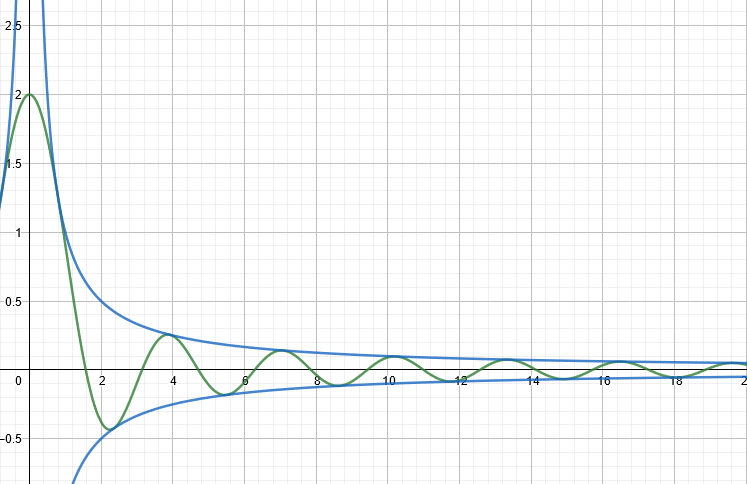
\includegraphics[width=\linewidth]{Images/majorante}
	\end{minipage}%%% to prevent a space
	\begin{minipage}{0.25\textwidth}
		\noindent Wenn \underline{Majorante} Blau $g(x)$ \textbf{Konvergiert}, und Grün $f(x)$ in Blau eingeschlossen ist, dann muss Grün auch konvergieren.
	\end{minipage}
\end{center}
\[\int g(x)dx \xrightarrow{\text{Konv.}} \int\left|f(x)\right| \xrightarrow{\text{Konv.}} \int f(x)dx \]

\begin{center}
	\begin{minipage}{0.2\textwidth}
		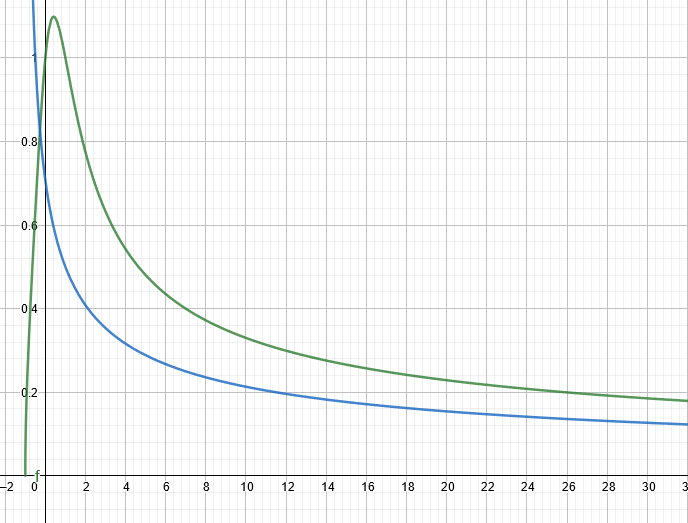
\includegraphics[width=\linewidth]{Images/minorante}
	\end{minipage}%%% to prevent a space
	\begin{minipage}{0.25\textwidth}
		\noindent Wenn \underline{Minorante} Blau $g(x)$ \textbf{Divergiert}, und Grün $f(x)$ nicht kleiner als Blau wird, dann muss Grün auch divergieren.
	\end{minipage}
\end{center}

